\chapter{	进入32位模式并导入C语言	}
作者给开发的操作系统起名字叫~纸娃娃操作系统——haribote os。
\section{	制作真正的IPL	}
制作一个可以称为真正的IPL(启动程序装载器),让启动区真正的开始装载程序。

\cs

因为磁盘最初的512字节是启动区,所以要装载下一个512字节的内容。
程序是在上一天的基础上修改的,添加了以下内容:

\dag |projects\03_day\harib00a|
\begin{code}[label=ipl.nas 本次添加的部分]
        MOV		AX,0x0820
		MOV		ES,AX
		MOV		CH,0			; シリンダ0
		MOV		DH,0			; ヘッド0
		MOV		CL,2			; セクタ2

		MOV		AH,0x02			; AH=0x02 : ディスク読み込み
		MOV		AL,1			; 1セクタ
		MOV		BX,0
		MOV		DL,0x00			; Aドライブ
		INT		0x13			; ディスクBIOS呼び出し
		JC		error
\end{code}

|INT 0x13|是调用BIOS的0x13号函数。

下面是BIOS 13中断的简单说明(功能有磁盘的读、写、扇区校验、寻道)
\begin{itemize}
  \item AH=0x02 读盘/0x03写盘/0x04校验/0x0c寻道
  \item AL=处理连续扇区数
  \item CH=柱面号\&0xff
  \item CL=扇区号(0$\sim$5位)\verb`|`(柱面号\&0x300)$\gg$2
  \item DH=磁头号
  \item DL=驱动器号
  \item ES:BX=缓冲地址
\end{itemize}

返回值:FLAGS.CF=0,没有错误AH=0;FLAGS=1有错误,AH保存错误码

这里,JC(jump if carry)是条件跳转指令,如果进位标志为1,就跳转。跳转条件看调用函数的返回值FLAG.CF。

对照程序和BIOS函数参数说明,可以知道我们这次使用的是读盘,柱面号是0,磁头号是0,扇区号是2,磁盘号是0。
\cs

\begin{figure}[!ht]
  \centering
  % Requires \usepackage{graphicx}
  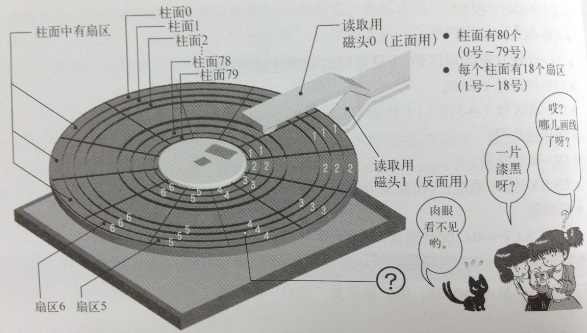
\includegraphics[width=0.6\textwidth]{day03-ruanpan.jpg}\\
  \caption{软盘的结构}\label{ruanpan}
\end{figure}

一张软盘有80个柱面,2个磁头,18个扇区,且一个扇区有512字节。所以一张软盘的容量是$80\times 2\times 18\times 512=1474560 Byte= 1440KB$。

含有IPL的启动区,位于C0-H0-S1(柱面0,磁头0,扇区1),下一个扇区是C0-H0-S2,这次我们要装载的扇区就是这个。

ES:BX=缓冲地址~是个内存地址,表明要把软盘上读出的数据装载到内存的哪个位置。由于一个BX只能表示0$\sim$0xffff的值,即64K,太小了,使用段寄存器以ES:BX这种方式来表示地址,写成“MOV AL,[ES:BX]”,代表“ES$\times$16+BX”的内存地址。程序中指定了ES=0x0820,BX=0,所以软盘的数据会被装载到0x8200$\sim$0x83ff的位置。
\cs

作者使用变量的方式改写了Makefile文件,可以看一下。

\section{	试错	}
鉴于软盘的不可靠性,有时候需要在软盘读不出来的时候多读几次,这里重读5次。

\dag|projects\03_day\harib00b|
\begin{code}[label=ipl.nas 本次添加的部分]
; ディスクを読む

		MOV		AX,0x0820
		MOV		ES,AX
		MOV		CH,0			; シリンダ0
		MOV		DH,0			; ヘッド0
		MOV		CL,2			; セクタ2

		MOV		SI,0			; 失敗回数を数えるレジスタ
retry:
		MOV		AH,0x02			; AH=0x02 : ディスク読み込み
		MOV		AL,1			; 1セクタ
		MOV		BX,0
		MOV		DL,0x00			; Aドライブ
		INT		0x13			; ディスクBIOS呼び出し
		JNC		fin				; エラーがおきなければfinへ
		ADD		SI,1			; SIに1を足す
		CMP		SI,5			; SIと5を比較
		JAE		error			; SI >= 5 だったらerrorへ
		MOV		AH,0x00
		MOV		DL,0x00			; Aドライブ
		INT		0x13			; ドライブのリセット
		JMP		retry
\end{code}

其中,JNC(jump if not carry),进位标志为0的话跳转;JAE(jump if above or equal),大于或等于时跳转。

在重新读盘之前,做了如下处理,AH=0x00,DL=0x00,INT=0x13,即完成系统复位。
\section{	读到18扇区	}
往后多读几个扇区,读完柱面0的18个扇区。

\dag|projects\03_day\harib00c|
\begin{code}[label=ipl.nas 本次添加的部分]
; ディスクを読む

		MOV		AX,0x0820
		MOV		ES,AX
		MOV		CH,0			; シリンダ0
		MOV		DH,0			; ヘッド0
		MOV		CL,2			; セクタ2
readloop:
		MOV		SI,0			; 失敗回数を数えるレジスタ
retry:
		MOV		AH,0x02			; AH=0x02 : ディスク読み込み
		MOV		AL,1			; 1セクタ
		MOV		BX,0
		MOV		DL,0x00			; Aドライブ
		INT		0x13			; ディスクBIOS呼び出し
		JNC		next			; エラーがおきなければnextへ
		ADD		SI,1			; SIに1を足す
		CMP		SI,5			; SIと5を比較
		JAE		error			; SI >= 5 だったらerrorへ
		MOV		AH,0x00
		MOV		DL,0x00			; Aドライブ
		INT		0x13			; ドライブのリセット
		JMP		retry
next:
		MOV		AX,ES			; アドレスを0x200進める
		ADD		AX,0x0020
		MOV		ES,AX			; ADD ES,0x020 という命令がないのでこうしている
		ADD		CL,1			; CLに1を足す
		CMP		CL,18			; CLと18を比較
		JBE		readloop		; CL <= 18 だったらreadloopへ
\end{code}

JBE(jump if below or equal),小于等于则跳转。

要读入下一个扇区只需给CL加1,给ES加上0x20(512/16)。CL是扇区号,ES指定读入地址。

这里使用循环的方式读入各个扇区,而不是在开始的时候设置读入的扇区数AL=17,因为磁盘BIOS读盘函数有一些“补充说明”:
\begin{quote}
  指定处理的扇区数,范围在0x01~0xff(指定0x02以上的数值时,要特别注意能够连续处理多个扇区的条件。如果是FD的话,似乎不能跨越多个磁道,也不能超过64KB的界限。)
\end{quote}

经过上面这些读盘处理,已经把磁盘上C0-H0-S2到C0-H0-S18的$512\times 17=8704$个字节的内容,装载到了内存的0x8200$\sim$0xa3ff。
\section{	读入10个柱面	}
\section{	着手开发操作系统	}
\section{	从启动区执行操作系统	}
\section{	确认操作系统的执行情况	}
\section{	32位模式前期准备	}
\section{	开始导入C语言	}
\section{	实现HLT(harib00j)	}
